\subsection{Network}

% "To help deal with this complexity, network designers have developed general blueprints — usually called network architectures — that guide the design and implementation of networks, the central ideas that are common to all network architectures." \cite{book:net-sys}
% *Internet Architecture* - "We call the set of rules governing the form and content of a protocol graph a network architecture."~\cite{book:net-sys}

% "Muitas questões estão envolvidas para que esta conversa entre os computadores possa tornar possível tudo o que queremos.
% Sua complexidade é tão grande e são tantos os problemas, que as primeiras pessoas que estudaram a questão optaram por adotar a máxima “dividir para governar”.
% Sendo assim, não existe uma única conversa, mas várias conversas, cada uma buscando resolver um problema na comunicação entre os computadores.

% E por serem essas conversas previamente acertadas, isto é, cada pergunta possui respostas preestabelecidas, elas são denominadas protocolos [de comunicação].

% Os protocolos servem então para que vários computadores e redes conversem entre si de maneira ordenada."



% is commonly believed that P2P networks
% In theory, as the number of peers increases,
% PQ ISSO NÃO ACONTECE?!


% Pq overlay... [Como chegou de P2P a overlay?]
"Overlay networks provide exactly this opportunity [of disruptive technology].
Overlay nodes [há alguma diferença para "conventional nodes"? Qual o significado disso na blockchain?] can be programmed to support the new capability or feature and then depend on conventional nodes to provide the underlying connectivity.
~~Over time, if the idea deployed in the overlay proves useful, there may be economic motivation to migrate the functionality into the base system—that is, add it to the feature set of commercial routers.
On the other hand, the functionality may be complex enough that an overlay layer may be exactly where it belongs."~~\cite{book:net-sys}
% *Over time, blockchain third generation...*

"Keep in mind that even though these nodes are neighbors in the ID space, they are likely to be physically distributed across the Internet.
Thus, while a power outage in an entire city might take down physically close replicas of a file in a traditional file system, one or more replicas would likely survive such a failure in a P2P network."~\cite{book:net-sys}
















\dots

They
have been varying between centralized and decentralized use of computing power, storage, infrastructure, protocols, and code since its advent~\cite{LFS171x}.
``Massive data sets, which are housed on mainframes, could move onto a distributed architecture. This data could replicate from server to server, and subsets of the data could be accessed and processed on clients, and then, synced back to the server (\textit{Is distributed DB or processing?}).
Over time, Internet and cloud computing architectures enabled global access from a variety of computing devices; whereas mainframes were largely designed to address the needs of large corporations and governments. Even though this 'cloud architecture' is decentralized in terms of hardware, it has given rise to application-level centralization (e.g. Facebook, Twitter, Google, etc). ((\textit{app-level is a network term...}))
Currently, we are witnessing the transition from centralized computing, storage, and processing to decentralized architectures and systems.''~\cite{LFS171x}

``Distributed ledger technology is ONE OF the key innovations making this shift possible (\textit{what the others?}).''~\cite{LFS171x}.
``There are similar technologies to blockchain, but since all these definitions and concepts relating to these technologies ultimately refer to databases which are distributed, the term DLT is commonly used as a term of art by those in the technology development community as the generic descriptor for any distributed, encrypted database and application that is shared by an industry or private consortium, or which is open to the public.[ver ref 5]''~\cite{itu2017}


% 25/04/18
% O que é a computação em nuvem? - https://aws.amazon.com/pt/what-is-cloud-computing/
% Is Fog Computing The Next Big Thing In Internet of Things? - https://www.forbes.com/sites/janakirammsv/2016/04/18/is-fog-computing-the-next-big-thing-in-internet-of-things/#2239238d608d
% Distributed Database Architecture - https://docs.oracle.com/cd/B28359_01/server.111/b28310/ds_concepts001.htm#ADMIN12074

\begin{figure}[h!tb]{\textwidth}
  \caption{Types of databases.} \label{fig:DBs}
  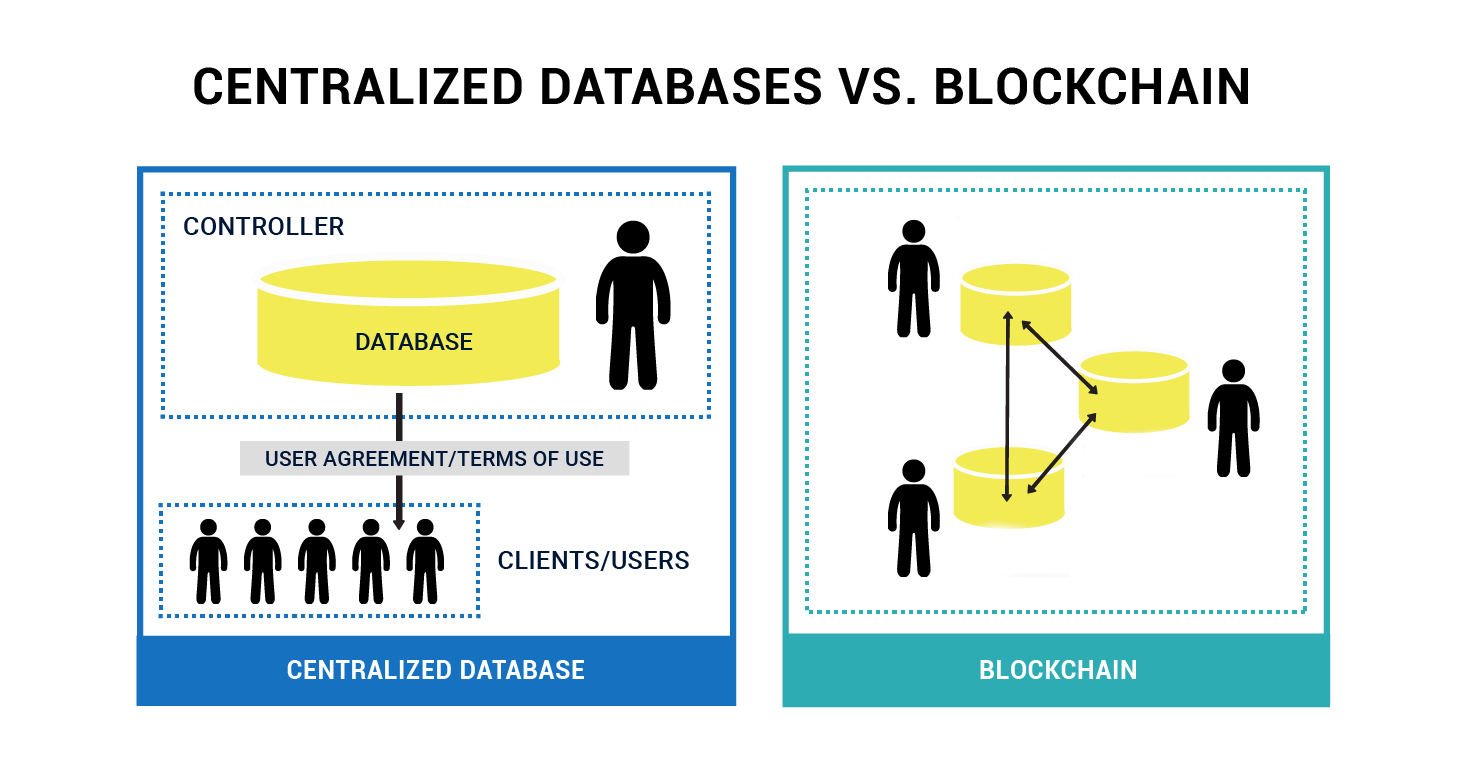
\includegraphics[width=0.5\textwidth]{pics/db}
  \legend{``blockchain is data-centric network''[Holochain ``definition'']}
  \source{\citeonline{LFS171x}}
\end{figure}

% "To understand how BitTorrent functions, first consider how normal downloading works. Personal computers connected to the Internet are known as clients while the websites visited reside on Internet servers. Servers "serve up information" to clients. If you surf to a site and click on a link to download a program, you create a one-on-one connection to that server that uses whatever bandwidth is necessary to serve you the file. When you have received the entire file, the connection is released so the server can utilize that stream of bandwidth for handling other connections.
% The problem arises when unusually high numbers of clients visit a site simultaneously. This can cause the server to effectively run out of available bandwidth and "crash." When this happens, clients are refused a connection. "The site is down."
% To avoid this, BitTorrent creates a different networking scheme. It uses the other clients who are also downloading the file to effectively act as servers to one another, simultaneously uploading the parts of the file received to others requesting the file. Hence, when you click on a file to download, several connections will be made to receive "slices" of the file that combine to create the entire file. Meanwhile, as you are downloading these "slices" you are also uploading them to anyone else that needs the parts you are receiving. Once the entire file is received it is considered polite to keep your client connected to act as a seed. A seed refers to a source that has the entire file available.
% In this way BitTorrent relieves the burden of the servers but more significantly it makes it possible for anyone to disseminate a file quickly and easily without requiring expensive servers or an infrastructure of distribution. If the demand is there, the file will spread.
% BitTorrent differs from other peer-to-peer (P2P) programs like Kazaa or Morpheus in that you do not make a
% library of files available for sharing. You only share the file you are actively receiving (or have just finished
% receiving)."
% https://drive.google.com/file/d/12ykI12uVwWCIr_QhXQw4z1WZF6cXQmJh/view

% ---------
% CS x P2P
% ---------

% -------------------------------------
% data structure x network architecture
% -------------------------------------
% https://en.wikipedia.org/wiki/Data_structure
% https://en.wikipedia.org/wiki/Network_architecture
% Tem fins diferentes, mas como estão se relacionando na blockchain? Falar sobre eles em separado?

\subsection{What is a DLT?}
% Como o banco de dados funciona em uma arquitetura p2p!

\begin{quotation}
A distributed ledger is a type of data structure which resides across multiple computer devices, generally spread across locations or regions.

Distributed Ledger Technology includes blockchain technologies and smart contracts. While distributed ledgers existed prior to Bitcoin, the Bitcoin blockchain marks the convergence of a host of technologies, including timestamping of transactions, Peer-to-Peer (P2P) networks, cryptography, and shared computational power, along with a new consensus algorithm. 

In summary, distributed ledger technology generally consists of three basic components:
\begin{itemize}
\item A data model that captures the current state of the ledger (\autoref{ssec:block-design})
\item A language of transactions that changes the ledger state (\autoref{ssec:smart-contract})
\item A protocol used to build consensus among participants around which transactions will be accepted, and in what order, by the ledger (\autoref{ssec:consensus}).
\end{itemize}
\end{quotation}~\cite{LFS171x}

``DLT has the potential to speed up and reduce the cost of transactions, give individuals more control over their personal data, reduce or remove the need for costly intermediaries, provide secure ‘smart’ legal contracts that execute without user intervention, bolster data security by providing almost real-time evidence of tampering, and revolutionize regulatory compliance.''~\cite{itu2017}

``DLTs generally integrate a number of innovations which include: Database (ledger) entries that cannot be reversed or otherwise modified, the ability to grant granular permissions, automated data synchronization, rigorous privacy and security capabilities, process automation, and transparency, such that any attempts at changes to entries will notify others. Its main disruptive attribute is that it is decentralized and therefore not dependent on a central controller or storer of the data.''~\cite{itu2017}

``These innovations also prompt a number of challenges related to their implementation, including the nascent (and often not yet properly stress-tested) nature of the technologies used; uncertain legal and regulatory status; privacy and confidentiality issues; cultural changes in requiring users to have ‘trust’ in often anonymous counterparties; scalability of the DLTs for mainstream use comparable to and exceeding existing non-DLTs performing similar functional''~\cite{itu2017}

``A prime example of DLT is called blockchain technology. All blockchains operate by taking a number of records and putting them in a block and then chaining that block to the next block using a cryptographic signature. While the data (blocks) are stored one after the other in a continuous ledger, they can only be added when the participants reach a quorum (consensus) over their validity. Each record is time/date stamped and provided with a unique cryptographic signature, which is designed to ensure the authenticity and integrity of the ledger. This distributed design eliminates the need for a central authority or intermediary to process, validate, or authenticate transactions and data.''~\cite{itu2017}

``The manner in which consensus for proposed changes to the ledger is reached defines the type of blockchain. The process may be permissionless or permissioned. Some may be public or private and may allow only certain people to view all or subsets of the data on a blockchain. These ledgers are similarly designed for rapid detection of unauthorized changes to the data.''~\cite{itu2017}

``Usually only those with an appropriate cryptographic key can view or add to the data on a blockchain, which may layer on permissions for different types of users where necessary.9 Anyone can, with the right tools, create a blockchain and decide who can see the data in the blockchain, or add data to it. Banks, governments, and private entities are rapidly developing''~\cite{itu2017}


\subsection{I see cryptography everywhere}

"Transactions represent state transitions with ownership information, which could include new data records and transfer of control among participants.
The integrity of the transactions is ensured by cryptographic techniques.
The transaction is sent to a node connected to the blockchain network, which knows how to validate the transaction.
When a transaction reaches a mining [qual seria o termo mais generalista?] node, it is verified and included in a block, which is propagated to the network."~\cite{xu2016}

"How it works is that a standard algorithm is run over a file (any file) to compress it into a short 64-character code (called a hash) that is unique*
% pegar no ebook que está no Windows
to that document."~\cite{swan2015blockchain}


\subsection{Smart-contracts: blockchain programming language~\label{ssec:smart-contract}}
% \section{smart contracts: blockchain code protocol}
% Fale e dê exemplos sobre o Solidity (fale um pouco sobre Ethereum). Fale um pouco e dê exemplos de códigos escritos no NEO (C# / python). Essa parte posso te ajudar a aprofundar, inclusive a descrever melhor a máquina virtual deles. O ideal seria também falar o HyperLedger e do Fabric da IBM. Tudo isso pode ser mais por alto por agora, e deixar mais detalhes pra versão final da tese.



\subsection{Consensus: ledger management protocol~\label{ssec:consensus}}
% just to use right words: https://pt.wikipedia.org/wiki/Simple_Network_Management_Protocol



\subsection{Distributed ledgers types}

``blockchain technology has some key differentiators from databases.
A blockchain is a write-only data structure, where new entries get appended onto the end of the ledger. Every new block gets appended to the block chain by linking to the previous block's 'hash'.
There are no administrator permissions within a blockchain that allow editing or deleting of data.
In a \href{https://en.wikipedia.org/wiki/Relational_database}{relational database}, data can be easily modified or deleted. Typically, there are database administrators who may make changes to any part of the data and/or its structure. Additionally, blockchains were designed for decentralized applications, whereas relational databases, in general, were originally designed for centralized applications, where a single entity controls the data''~\cite{LFS171x}.

Therefore, the blockchain technology has been designating as \emph{permissionless} and as \emph{permissioned}~\cite{itu2017,peck2017}.
Although both are ``similarly designed for rapid detection of unauthorized changes to the data''~\cite{itu2017},
the latter aims to overcome some challenges presented on the former~\cite{peck2017}.
There is a belief that this categorization may be more granular~\cite{itu2017},
even so, its range by what is shown in Table \ref{tab:blocks-classif} so far.

The unique characteristic of this technology architecture by privacy levels has been allowing the development of several new applications accordingly with specific needs.
For some purposes, its use can be interpreted merely as a cloud computing service improvement,
wherein ``abstractions over the lower-level technical details is key to provide rapid experimentation with [the technology], to support businesses in their desire to explore its potential''~\cite{singh2017}.

For instance, a permissioned private blockchain, also referred as \acrfull{baas}, can be easily compared with a secure append-only database,
with similar ``functionalities as a standard cloud-hosted application, with suitable access control and identity regime, that records specific actions of those involved in an appropriate `secure' database''~\cite{singh2017}.
However, it lacks the sense of self-organized community in a trustfulness environment~\cite{peck2017}.

% \input{block-table.tex} % tem tabela boa em xu2017

``All blockchains operate by taking a number of records and putting them in a block and then chaining that block to the next block, using a cryptographic signature.20 The method used to validate the accuracy of a distributed ledger is known as ‘consensus.’21''~\cite{itu2017}

``The manner in which consensus for proposed changes to the ledger is reached defines the type of blockchain. (Depending on the DLT, the consensus method may be called Proof of Stake (POS), or Proof of Work (POW). For example, with cryptocurrencies POS is a consensus mechanism used as an alternative to the POW mechanism used in Bitcoin. POS cryptocurrencies are ‘minted’ rather than ‘mined,’ so avoiding expensive computations and thus providing a lower entry barrier for block generation rewards. For a fuller discussion of these differences, see Bitfury Group (2015) Proof of Stake Versus Proof of Work, available at \url{https://goo.gl/ebS2Vo}.)''~\cite{itu2017}

``Distinctions between permissioned and permissionless described here reflect the current state of the art. As DLTs mature, many believe that there will be a full spectrum between permissioned and permissionless.''
Is clear defined on~\cite{uk2016}.

``Public blockchains are said to be fully decentralized.''~\cite{itu2017}

% \cite{xu2017} % Blockchain Taxonomy --> usar como base para comparar as blockchains mais conhecidas atualmente
% Link with
% IEEE spectrum magazine - p. 27(types of proofs), 29(smart contract), 35types of blocks)
% UK report
% PwC (do SBPO) - p. 7 (Dapps, tokens, proofs)
% itu2017 (tópico :'DLT design')
% all reports related with classifications of purpose


\subsection{Blockchain designs~\label{ssec:block-design}}

``While there are still significant challenges in the development and implementation of DLTs, many incorporate some or all of the following design features''
\begin{descriptive}
	\item cryptographic techniques to reach consensus on data entry and accuracy
    \item scalability
    \item transparency of data entry
    \item authentication of the entry of data
    \item disintermediation of trust
    \item replication of data to avoid single point of failure
    \item immutability of the data record
    \item evidence of tampering
    \item borderless
    \item quick to update
    \item permanent uptime
    \item access control \& authentication through cryptographic keys
    \item smart, self-executing contracts.
\end{descriptive}
~\cite{itu2017}.

-- Talk about architecture

\begin{figure}[!ht]{\textwidth}
  \caption{Basic blockchain architecture.} \label{archain}
  
\includegraphics[width=5cm]{config/logo_uerj_cor.jpg}
%   \legend{Texto da legenda.}
  \source{Modified from~\citeonline{xu2016}.}
\end{figure}

% \hrule



% \subsection{Estruturas de dados}
% \subsection{Redes de computadores}
% \subsection{Confiança e troca de favores}
% \subsection{Segurança, de quem e por quem}
% \subsection{Blockchain em essência}

\subsection{Initial Coin Offering (ICO) basics~\label{sec:ico}}
% conceitos de tokens/criptomoedas (citar a primeira ICO brasileira da Niobium que foi feita dentro da legislação brasileira para a BOMESP, bolsa de moedas de SP).

% \subsection{tokens/criptomoedas}
% \subsection{Análise de mercado, demanda x oferta}
% \subsection{Solução de integração e desenvolvimento}
% \section{Aplicação real no caso brasileiro}

\section{Distributed applications on the electricity sector~\label{sec:blockchain}}

It is the innovative approach of \acrshort{dlt} that enables diversified experimentation models,
such as the case with \acrshort{gd}, mainly with decentralized solar energy networks~\cite{its3}.
However, the technology configuration range capability also allows the blockchain to be used throughout the whole energy sector chain, as synthesizes the Figure \ref{fig:block-on-energy}.

The electricity network use to have a top-down business model with utilities and big power generators sending electricity to customers.
Directly trade of electricity between generators and residential consumers is already a reality in the European Union (EU)~\cite{blocktrading,Brasil-futuroEE},
whilst in Brazil its mechanism is limited by the level of power consumption, and not by consumer class.
% However, the complete unbundling of the sector has been expected for a while~\cite{iea2011,epe2014}, at the same time as technology has been evolving to allow its happening, such as the case with blockchain technology, that can be a tool to standardize this market.

% TALVEZ ISSO JÁ TENHA SIDO DITO NA SEÇÃO 2!
With increase adoptions of \acrshort{gd}, the electricity direction goes in both ways, with end consumers injecting power back to the grid~\cite{peck2017}.
It is a measured beyond the traditional \acrfull{b2c} energy trading,
in which the emerging market of \acrshort{p2p} electricity exchange between end consumers,
and between them and local distribution utility could improve current trade model towards a more challenge one.

Nonetheless, the \acrshort{p2p} market itself is a mystery for everyone.
The case running in EU is similar to the \acrshort{acl} model in Brazil, but prosumers and consumers can not directly exchange electricity indeed.
There are no direct involvement between residential consumers, in a smaller time scale and without an intermediary party.

Although the consumers can save on the power generation rate, they still can not profit with their investment.
The \acrshort{gd} market is still restricted but it could behave as the free-trade at \acrshort{acl}.
Perhaps one of the biggest problems, aside from technical factors,
it is ensuring energy transactions by countless people who do not know each other and have particular power needs.

In this context,
new technologies to exchange of information and to allow interactions between different autonomous agents % agentes? conflito de nomenclatura com agentes do setor elétrico REVER!!!
embedded with artificial intelligence tools, and mechanisms such as blockchain, should be a feasible solution and a trend for the next few years~\cite{Coelho2017MAS}. %[ Coelho et al., 2017].
% The presence of prosumers into the electricity market sustained by blockchain allows the share and update of data by multiple unknown parties in a trusty and verified manner~\cite{peck2017,wec2017}.
As a result, the blockchain projects can overcome the challenges with decentralized energy systems optimization,
leaving new approaches to arise, such as real-time pricing, consumers awareness about personal power consumption, prosumers awareness about when their generation is most needed, and social awareness about its impact on the grid~\cite{peck2017,wec2017}.

From this premise, solutions are being developed to enable the active participation of consumers in the electricity market.
In other words, leaving a position of just accumulate energy credits to an active position, in which the excess power generated could be converted into profit. % clearing = compensação!!!


% \begin{figure}[h!tbp]
%     \centering
%     \frame{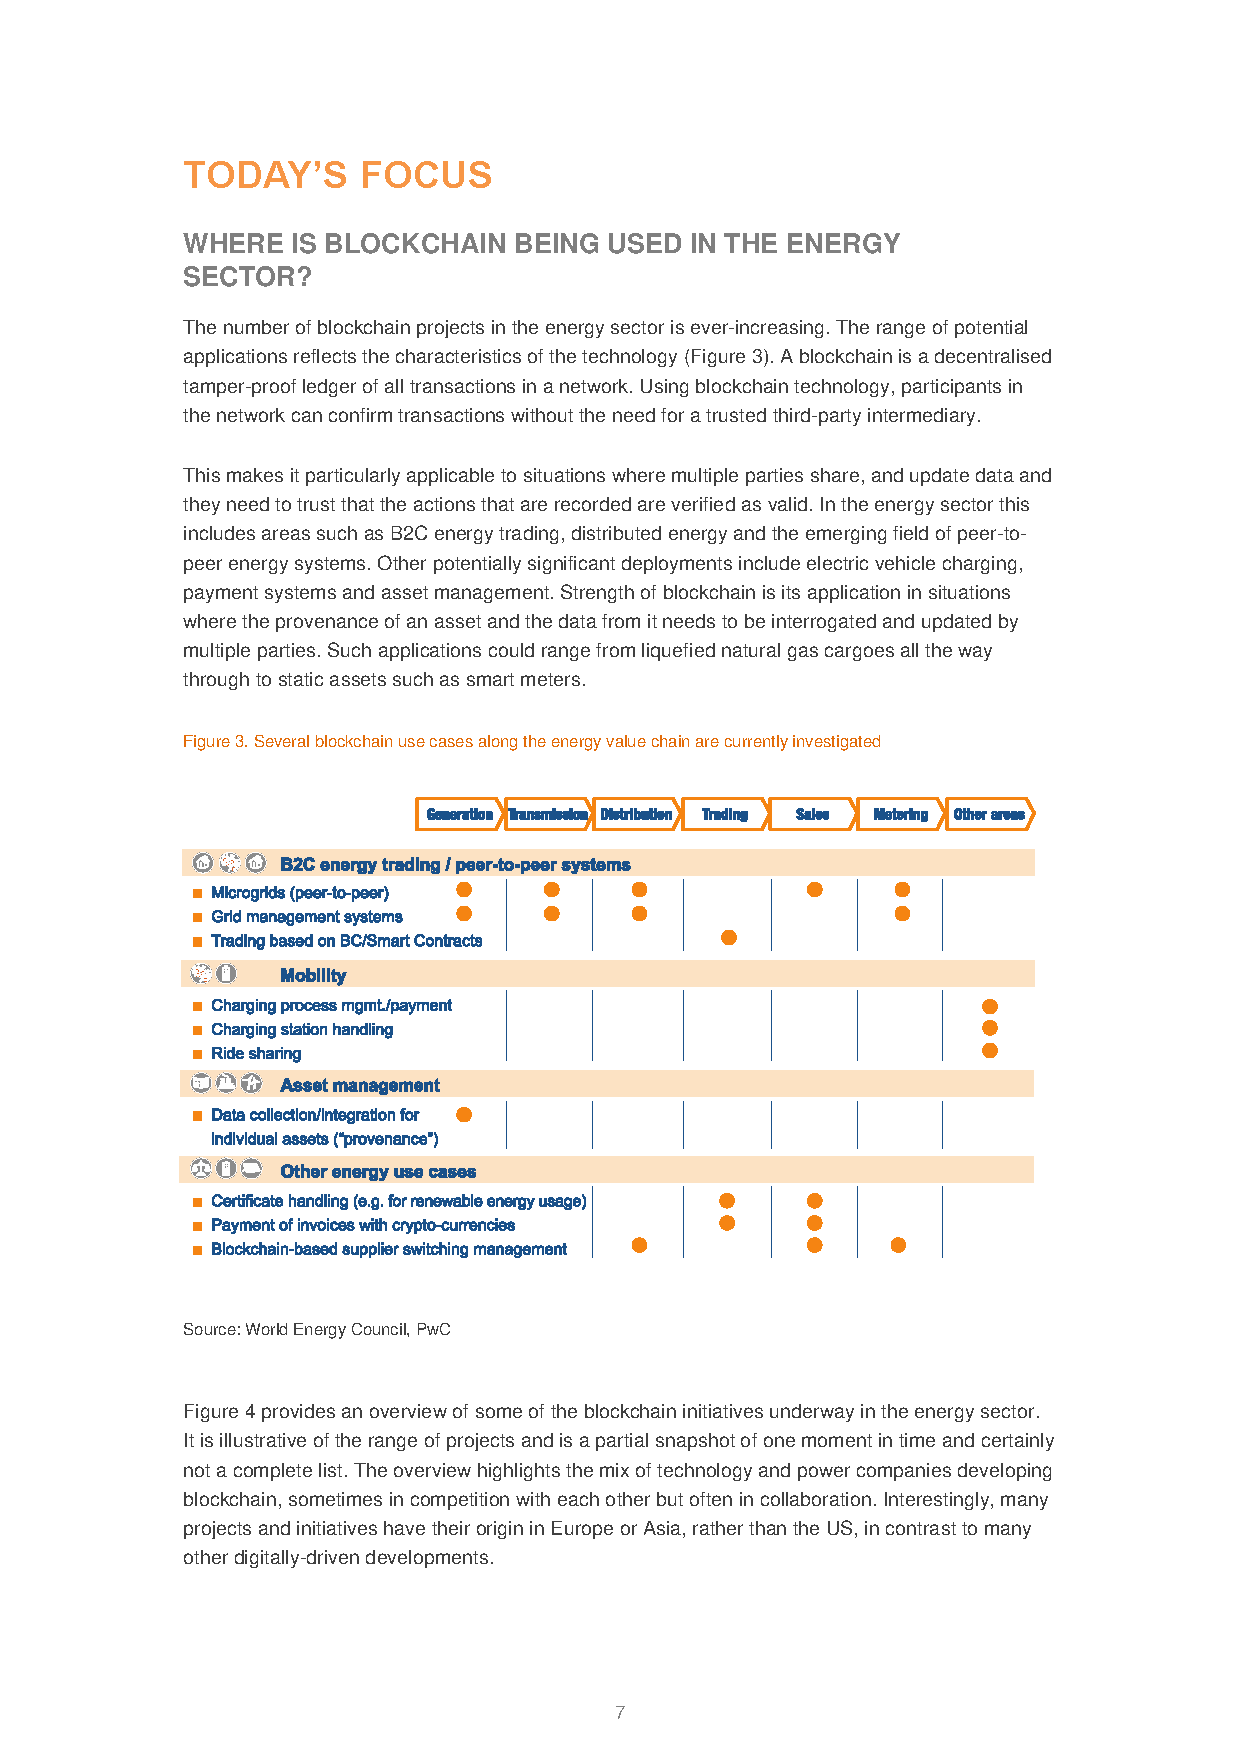
\includegraphics[clip, trim=3cm 7cm 3.25cm 13.25cm, width=\textwidth]{block-on-chain.pdf}}
%     \caption{Blockchain applications on electricity sector chain \textcolor{red}{(source:~\cite{wec2017})}.}
%     \label{fig:block-on-energy}
% \end{figure}

\subsection{New electricity market proposals~\label{sec:propostas}}

In a more simple and international way, the \emph{SolarCoin} is a digital asset that rewards owners of solar power generation, being basically a technology to encourage decentralized, clean, and renewable energy generation,
which aims to reduce the payback time for the solar installations~\cite{mit-dci}.
Its crypto-currency \emph{solarcoin (SLR)} works similarly to credit cards miles program, 1 MWh is equivalent to 1 SLR.

In the other hand, the Marubeni company is allowing Bitcoin payments options for electricity consumption in some regions of Japan~\cite{groarke2016}.
While a real case application in South Africa uses Bitcoin transfer for accounting clearing of electricity pre-paid system \textcolor{red}{[como citar um vídeo?]}.
% https://www.youtube.com/watch?v=cpMwPhA9QzM&feature=youtu.be&t=1h33m5s

In Dhaka, Bangladesh, the \emph{ME SOLshare Ltd} is a social enterprise that offer \acrshort{p2p} trade system for solar power generation, and finance photovoltaic installations for low-income families.
Founded in 2014, the SOLshare operates off-grid electricity in rural areas and allows its users to earn an income directly from the energy of the Sun.
Its goal is to empower people to become entrepreneurs, enabling the creation of a bottom up smart grid, and being ready for the future integration to power network of the country \textcolor{red}{[ref?]}.
In a similar approach, the Alliander utility aims for ``real-time'' energy trade on the Island of Texel (Holland),
with smart meters linked to blockchain technology, a new business arise towards the wholesale market~\cite{groarke2016}.

In the case of the \emph{Brooklyn Microgrid}, it is still limited to some consumers in Brooklyn, New York.
The owner of a PV power can sell its generation to a neighbor using a smart contract available by the startup LO3~\cite{blocktrading}. % [Merz , 2016]
But this model still faces regulatory issues of energy transaction, since it is under the concession area of different distribution utilities~\cite{mengelkamp2018}, which can not occur in Brazil as stated by \acrshort{gd} legislation.

In Australia, \emph{Power Ledger} goes a little further into the \acrshort{p2p} interaction, allowing the transaction between the units of a building with other consumers of the distribution grid, thanks to its tight relationship with local utility.
Owners of a \acrshort{gd} can decide for who they want to sell their surplus energy and at what price.
In the platform provided there is a mechanism of negotiation and clearing that is transparent, auditable and automated in the benefit of prosumers and consumers~\cite{pwrledger}.
They have already expanded to Auckland area, New Zealand, with expectations that schools, community groups and residential houses participate actively in the initiative~\cite{groarke2016}.

Other actions are taking place on different uses of electricity as well.
% For instance, \emph{Fortum} enables consumers to manage theirs home consumption over internet
% Fortum - Finland --> não achei a prov no site da empresa!
% "Fortum aims to enable consumers to control appliances over the internet in connected homes and view blockchains as micro demand response enabler at the device level."\cite{groarke2016}
For instance, the \emph{Wien Energie} utility uses the distributed technology to optimize and to save costs of gas trading for power generation~\cite{groarke2016}.
Established in Austria, the system is used to guarantee the stability of the grid in case the Sun or the wind does it not~\cite{wien-energie2016}.
And in Germany, the \emph{RWE} together with the company \emph{Slock.it} uses the blockchain to manage electric vehicle recharge in public charging stations.
They use an accounting unit supported by different energy suppliers in order to provide vehicle drivers a standard method of payment.
The RWE system is based on the product \emph{BigchainDB} by Ascribe from Berlin, but it is not yet known how smart contracts are used for unlocking charging stations~\cite{blocktrading}.

Moreover, real market applications have been tested up by the CoLab,
an IDEO's hub for collaborative innovation, that designs human-centered projects.
They have built three prototypes to understand blockchain potential with electricity applications.
The Smart Solar %- https://www.ideocolab.com/prototypes/smartsolar
directly connects a solar panel to the blockchain network in order to tracks its generation, 
and automatically issue a personal digital Renewable Energy Certificate (REC).
The Shift %- https://www.ideocolab.com/prototypes/shift
is a marketplace to trade energy and a self-management device to operate under power rates flexibility.
And the Plug 'n' Paid %- https://www.ideocolab.com/prototypes/plugnpaid
is the power device manager for homes, which uses Artificial Intelligence (AI) to adjust preferences and behaviors of homeowners looking for power efficiency.
It also manages consumption, buys power in real time, and trades power with neighboring homes accordingly with pre-charge payment.











%================================================================================

% ------------------------------------OLD----------------------------------------
% (BaaS) aplicações internacionais/nacionais de energia + blockchain (Brooklyn microgrid, power ledger, ...);

The unique characteristic of blockchain architectures by privacy levels has been allowing the development of several new applications accordingly with specific needs.
For practitioner purposes, i.e. businesses and governments, the use of blockchain can be interpreted merely as a cloud computing service improvement.
As stated by \citeonline{singh2017}, the blockchain technology can be offered in terms of \acrfull{iaas}, \acrfull{paas} and \acrfull{saas}.
Even if a so restrictive application, a permissioned blockchain with ..., can be fully replaced by a ... [pegar no texto].
Nonetheless, offer blockchain benefits as part of a dedicated service sounds tempting for (almost-)permissioned applications.
% continue text until explain Baas term.


Whereas that public blockchains ... do/represent ..., its lacks scalability... , as previously commented.
Those concerns drive initiatives towards a not so open blockchain.

The ``Innovation Economy in the 2nd Era of the Internet'' for Canada government can be ... specifically for energy sector?~\cite{don2017}

Energy trading is one correlation infrastructure target by enterprises around the world, which advocate (and predict) for next-generation ... (? - rever texto)~\cite{sven2013}.

Furthermore, discussions under World Energy Council has being directed the role of blockchain for energy sector development~\cite{wec2017}.
% must be a paragraph to show applications


% Last application (02/05/18)
% https://www.ideocolab.com/prototypes/shift

Germany (\url{https://enerchain.ponton.de})
Enerchain is acting on high-voltage market (not on mini/microgrid until now), looking for replacement of usual power contracts between generators, utilities and traders.
TenneT, Sonnen, Vandebron and IBM are using blockchain to balance power dispatch across high-voltage grid, they're using DLT to manage power transmission. Nodes are substations, not final customers.

% 
\begin{quotation}
How is blockchain changing the energy markets? From peer-to-peer energy trading to tokenising the hardware, is a new wave of blockchain energy start ups leading us to a more sustainable, lower carbon economy?

This event showcases leading innovators in the field and explains to newcomers how to harness these technologies for the good of their business, and maybe even of the planet.

--- \href{https://unblockedevents.com/events/energy-unblocked/}{Energy Unblocked - Blockchain applications in the energy sector}. Key speakers:
\begin{itemize}
	\item Steven Campbell - CTO and Lead Developer, ElectriCChain
    \item Alpesh Doshi - Founder and CEO, Fintricity
    \item Joanna Hubbard - COO and Co-Founder, Electron
    \item Sunil Kumar - IBM
    \item Genevieve Leveille - Vice-Chair, techUK DLT working group
    \item Ismail Malik - Founder and CEO, Blockchain Lab and Editor in Chief, ICO Crowd magazine
    \item Emmanuel Marchal - Managing Director, Europe, ConsenSys
    \item Alastair Marke – Blockchain Climate Institute
    \item Sue McLean - FinTech Partner, Baker McKenzie
    \item Aleks Nowak - CIO of BlockEx
    \item Rodger Oates - Consulting Partner, Tata Consulting Services
    \item John Clippinger, Founder, Swytch
    \item Nick Beglinger, Cleantech21
\end{itemize}
\end{quotation}
% ------------------------------------OLD----------------------------------------

%================================================================================


%================================================================================
% EXEMPLOS DE USO

% \begin{figure ou table}[posição]{largura da figura}
%   \caption{Título da figura.} \label{rotulo}
%   
\includegraphics[width=\hsize]{config/logo_uerj_cor.jpg}
%   \legend{Texto da legenda.}
%   \source{Citação da fonte ou `O autor.'.}
% \end{figure}

% \begin{figure}[!ht]{11cm}
%   \caption{Título da figura.} \label{outro.rotulo}
%   \subfloat[][]{\label{subrotulo1}
%     \fbox{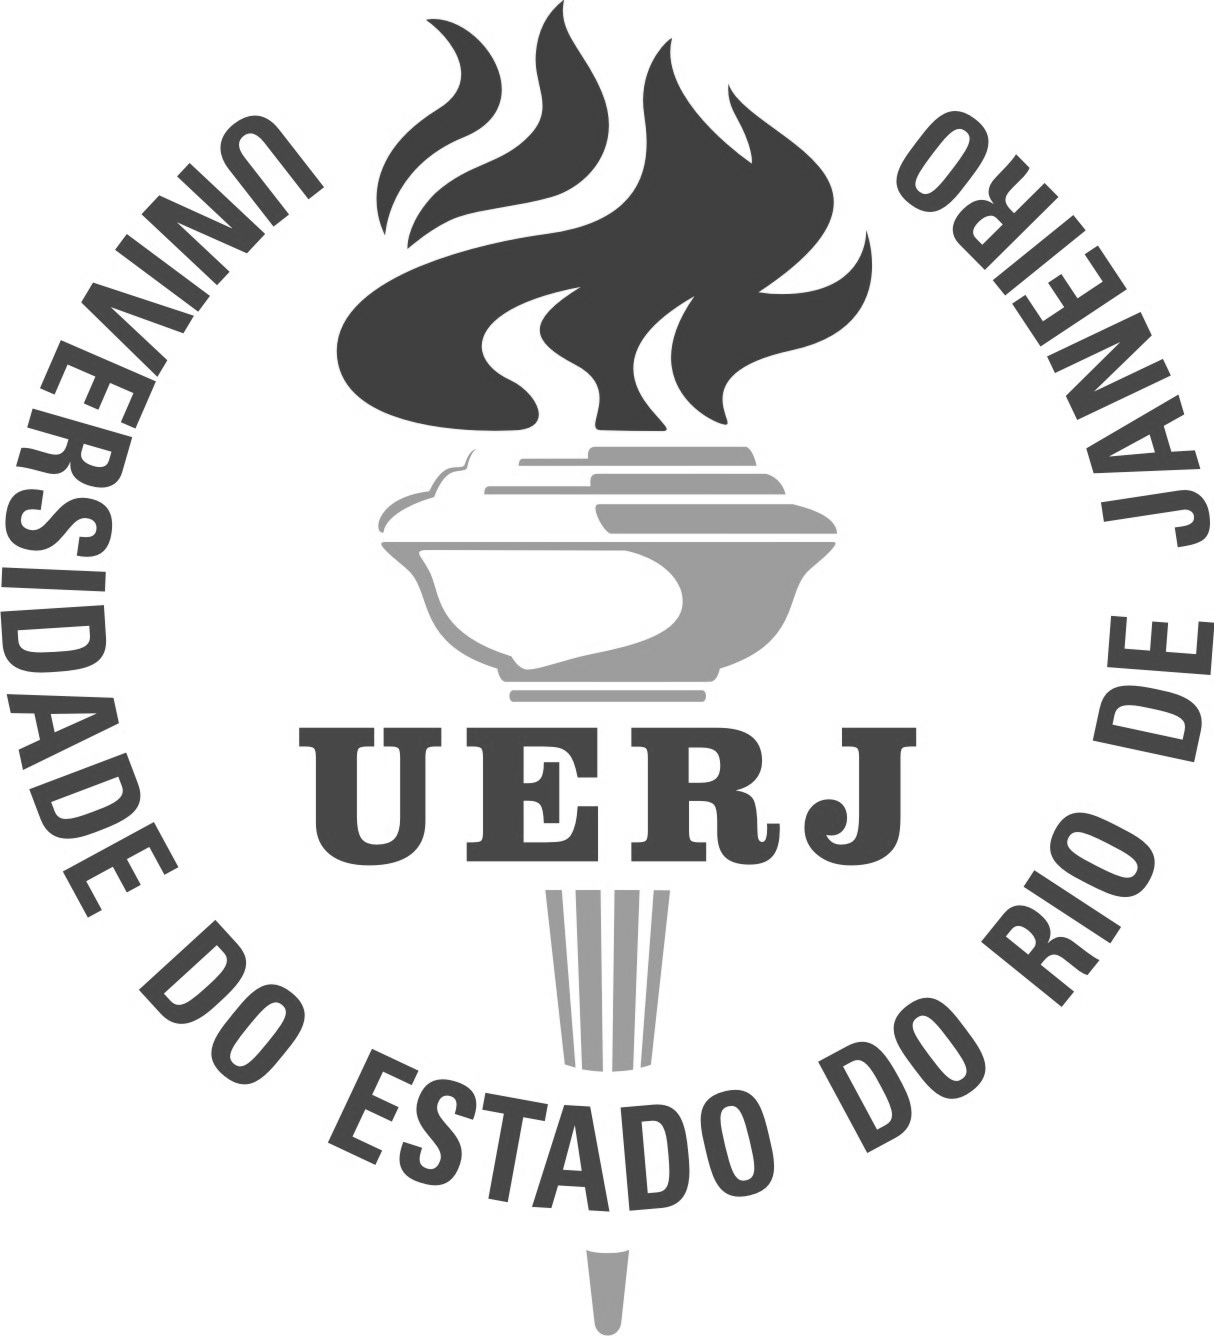
\includegraphics[width=0.45\hsize]{config/logo_uerj_cinza.png}}}\hfill
%   \subfloat[][]{\label{subrotulo2}
%     \fbox{
\includegraphics[width=0.45\hsize]{config/marcadagua_uerj_cinza.png}}}\\
%   \subfloat[][]{\label{subrotulo3}
%     \fbox{
\includegraphics[width=0.45\hsize]{config/logo_uerj_cor.jpg}}}\hfill
%   \legend{Texto da legenda. \subref{subrotulo1} Texto da imagem.
%           \subref{subrotulo2} Texto da imagem.
%           \subref{subrotulo3} Texto da imagem.}
%   \source{Citação da fonte ou `O autor'.}
% \end{figure}

\section{Challenges -- understand this topic}
``Current methods of data storage on centralized systems have always been vexed by attempted and successful intrusions.77 Database controllers attempt to harden these systems against data compromise and leak of private and confidential information through inter alia tightly controlling access through just one or more trusted (central) parties and by encrypting databases.78

With the distributed node motif embedded in the DNA of most DLTs, they have a different perspective to the storage of data and access thereto. That is, data on blockchains in large measure should be visible to everyone – the nodes79 ‒ on that blockchain.80 The ostensible reason for this is that to validate additions of data to the chain, nodes must have visibility over the data they are validating.81 In theory then, everyone could see everyone else’s data, at all times.

And, although access to a blockchain requires a private key, not all of the information on a blockchain is encrypted.82 For example, on the Bitcoin permissionless, public blockchain, data is pseudo-anonymous: The user’s ID is self-asserted and encrypted, but transactional data is not.

For financial institutions using permissioned, private blockchains, the visibility of commercially sensitive information – customers, transactions etc. – to everyone may be a serious barrier to adoption.83 So, although a blockchain could potentially replace Society for Worldwide Interbank Financial Telecommunication (SWIFT) 84 for value transfer or a bank for settlement, it also means that everyone could see the transaction flows, since they are on the nodes and ‒ intrinsically to the distributed nature of blockchain ‒ would have to verify any transactions for that transaction to be placed on the block.85

There is thus a tension between shared control of data on a ledger ‒ the core of the DLT motif ‒ and sharing of the data on a ledger.86

Solutions to these issues are being developed, but not yet mainstream. For example, ‘zero-knowledge proofs’87 are emerging, potentially enabling validation of data without visibility over the underlying data itself.

There is also R3’s Corda blockchain technology ‒ supported by over 70 banks and insurance companies worldwide – that shuns, in its design, global sharing of data such that only those parties with a legitimate need to know can see the data placed within an agreement on the blockchain.89

Digital Asset Holdings has also announced a ‘fingerprinting’ model to address privacy concerns: Though these fingerprints with blockchain data are shared amongst all users of a given blockchain, only trusted parties will be able to decipher them.90

And, for smart contracts, Hawk has been announced: It is a decentralized smart contract system that does not store financial transactions in the clear on the blockchain, retaining transactional privacy from the public’s view.91''\cite{itu2017}

``Despite the use of strong cryptography, DLTs are not necessarily a panacea for security concerns people may have.95 Indeed, there is a tradeoff between replacing costly – and often risky ‒ intermediaries with cryptographic key-only access distributed across nodes. 96 For example, for permissioned ledgers replacing centralized intermediaries, the cost-benefit in using blockchain is somewhat ameliorated by the need to trust permissioned authors rather than relying solely on the nodes who offer the guarantee of ledger integrity.97

The issues are said to be thus: The more trusted parties per node that are needed, so too does the compromisable 'surface area' of a distributed network increase.98 Also, requiring a third party private key management function is contradictory ‒ and possibly even nugatory ‒ to the core ‘disintermediation’ principles of DLTs. In all, these tradeoffs may arguably reduce the utility of DLTs.

Authorized access is also an issue: Nodes on the blockchain are – using current protocols – said to be unable to distinguish between a transaction by an authorized, actual user and a fake transaction by someone who somehow has gained access to the blockchain trusted party’s private key. 99 This means that if a bad actor gains access to a comprehensive banking blockchain that itself accesses all or of part of a core banking network blockchain ‒ or a real-time gross settlement system – then this breach would in effect be compromising all banks’ databases simultaneously.100

The ability then to upgrade the cryptographic techniques used for ‘old’ transactions should be considered in DLT designs.''\cite{itu2017}

``Continue on p. 24 (5.4)''\cite{itu2017}

